\documentclass[conference]{IEEEtran}
\usepackage[T1]{fontenc}
\usepackage{amsmath,amssymb}
\usepackage{booktabs}
\usepackage{tikz}
\usetikzlibrary{arrows.meta,calc,positioning}
\usepackage[hidelinks]{hyperref}

\newcommand{\code}[1]{\texttt{#1}}

% IEEEtran writes ``Abstract'' followed by an em dash; use a colon instead.
\usepackage{etoolbox}
\makeatletter
\patchcmd{\abstract}{---}{:\ }{}{}
\patchcmd{\abstract}{---}{:\ }{}{}
\patchcmd{\abstract}{---}{:\ }{}{}
\makeatother

\begin{document}

\title{SysMAC: A Verified $3 \times 3$ Output-Stationary\\Systolic Array for Signed 8-bit Matrix Multiplication}

\author{\IEEEauthorblockN{Abhishek Rana, Harshil Valecha, Sushant Yadav, Piyush, and Priyanshu Tomar}}

\maketitle

\begin{abstract}
This paper describes the design and verification of SysMAC, a $3 \times 3$ output-stationary systolic array that multiplies signed 8-bit matrices with 32-bit accumulation, written in Verilog-2001. Rows of one matrix and columns of the other enter the array with a one-cycle skew per row and column, so that each cell receives matching operand pairs, and a five-state controller sequences loading, a seven-cycle compute phase and result capture. One multiplication takes ten clock cycles. A sequential design with a single multiply-accumulate unit and the same interface takes 29 cycles, although the array uses nine multipliers to achieve this, and at this size only 43\% of its cell-cycles do useful work. The design is checked against an independent Python model of the array at the level of individual registers. All nine testbenches pass in simulation, and each of seven deliberately introduced design errors is detected. The results come from RTL simulation and a preliminary synthesis without timing; clock frequency and FPGA implementation are left for future work.
\end{abstract}

% ======================================================================
\section{Introduction}

The product $C = AB$ of two $N \times N$ matrices is
\begin{equation}
c_{ij} = \sum_{k=0}^{N-1} a_{ik}\, b_{kj},
\label{eq:matmul}
\end{equation}
which requires $N^3$ multiply-accumulate (MAC) operations. A fully connected neural network layer is one such product, and a convolution can be rewritten as one. A general-purpose processor evaluates \eqref{eq:matmul} with three nested loops and a single multiplier, fetching both operands from memory for every MAC.

A systolic array replaces the loops with a grid of identical cells. Operands enter at the edges and move one cell per clock cycle, so each value fetched from memory is reused by every cell it passes. This paper describes the design and verification of a small array of this kind. Our contributions are:
\begin{itemize}
\item a modular, synthesisable $3 \times 3$ output-stationary array with a frozen, documented interface;
\item a timing analysis that predicts the exact cycle count, cross-checked against a published closed-form model;
\item a sequential baseline with an identical interface, so that both designs run under the same tests;
\item a verification flow built on an independent register-level reference model, with mutation testing to show that the tests detect real design errors.
\end{itemize}

Section~\ref{sec:lit} reviews related work. Section~\ref{sec:design} presents the design, its analysis and the verification method. Section~\ref{sec:results} reports results, and Section~\ref{sec:future} discusses limitations and future work.

% ======================================================================
\section{Literature Review}
\label{sec:lit}

\subsection{Systolic arrays}
Kung and Leiserson introduced systolic arrays as special-purpose VLSI systems built from a few types of simple cells with regular, local connections~\cite{kung1978}. Their matrix multiplier is a hexagonally connected array for band matrices; we cite it for the concept rather than for the rectangular mesh used here. Kung later stated the central argument for the approach~\cite{kung1982}: because each input is used many times inside the array, the computation rate can be high while the input and output bandwidth stays modest. The same article identifies the properties that make such arrays practical: few cell types, only local wiring, and pipelining between cells.

\subsection{Systolic arrays in machine learning}
The Tensor Processing Unit (TPU) of Jouppi \emph{et al.}~\cite{jouppi2017} brought systolic arrays into production. Its matrix unit contains $256 \times 256$ MACs that perform 8-bit multiply-and-adds on signed or unsigned integers. Activations enter from the left, weights are loaded from the top, and 16-bit products are summed in 32-bit accumulators below the array. Accumulation therefore takes place outside the multiplier grid, whereas in our design each cell keeps its own sum.

The use of 8-bit operands with wide accumulators is supported by Jacob \emph{et al.}~\cite{jacob2018}, who show that networks can be trained for inference with integer-only arithmetic, using 8-bit weights and activations and 32-bit accumulation. SysMAC uses the same widths.

\subsection{Dataflow}
Chen, Emer and Sze~\cite{eyeriss2016} classify accelerators by the data that stays fixed inside a processing element: weight stationary, output stationary or no local reuse; they also propose row stationary. Sze \emph{et al.}~\cite{sze2017} survey these choices in a broader context. Samajdar \emph{et al.} apply the classification to systolic arrays in the SCALE-Sim simulator~\cite{scalesim2018} and later derive a closed-form runtime for each dataflow~\cite{scalesim2020}, which we use to check our timing in Section~\ref{sec:timing}. Gemmini~\cite{gemmini2021}, an open-source systolic generator, supports both output- and weight-stationary dataflows and illustrates the value of a clean separation between the processing element and the mesh, which we follow at a smaller scale.

\subsection{Position of this work}
The systems above are large and target convolution workloads. A $3 \times 3$ array cannot compete with them in throughput. Our goal is different: a small design in which every architectural claim, such as latency, operand alignment and accumulator range, is stated precisely and checked in simulation.

% ======================================================================
\section{Proposed Solution}
\label{sec:design}

\subsection{Specification}
Table~\ref{tab:spec} summarises the design decisions. All module interfaces are fixed in a shared port specification before implementation, so that the five modules could be developed and tested independently.

\begin{table}[t]
\caption{Design specification}
\label{tab:spec}
\centering
\begin{tabular}{@{}ll@{}}
\toprule
Parameter & Value \\
\midrule
Array size & $3 \times 3$ (array module parameterised in $N$) \\
Operands & signed, 8 bits \\
Accumulators & signed, 32 bits \\
Dataflow & output stationary \\
Input & $A$ and $B$ in parallel, 72 bits each \\
Output & all nine results in parallel, 288 bits \\
Packing & row major, element $(i,k)$ at bits $8(3i+k)$ upward \\
Clock and reset & single clock, synchronous active-high reset \\
\bottomrule
\end{tabular}
\end{table}

\subsection{Architecture}
Fig.~\ref{fig:top} shows the top level. When \code{start} is asserted, the input buffer latches both matrices and the array is cleared. The input scheduler then feeds the array for seven cycles, after which the output registers capture all nine accumulators. The output registers hold the result while the array is cleared for the next multiplication.

\begin{figure*}[t]
\centering
\resizebox{0.86\textwidth}{!}{% SysMAC top level (systolic_accelerator_top). Solid arrows: data.
% Dashed arrows: control from systolic_controller.
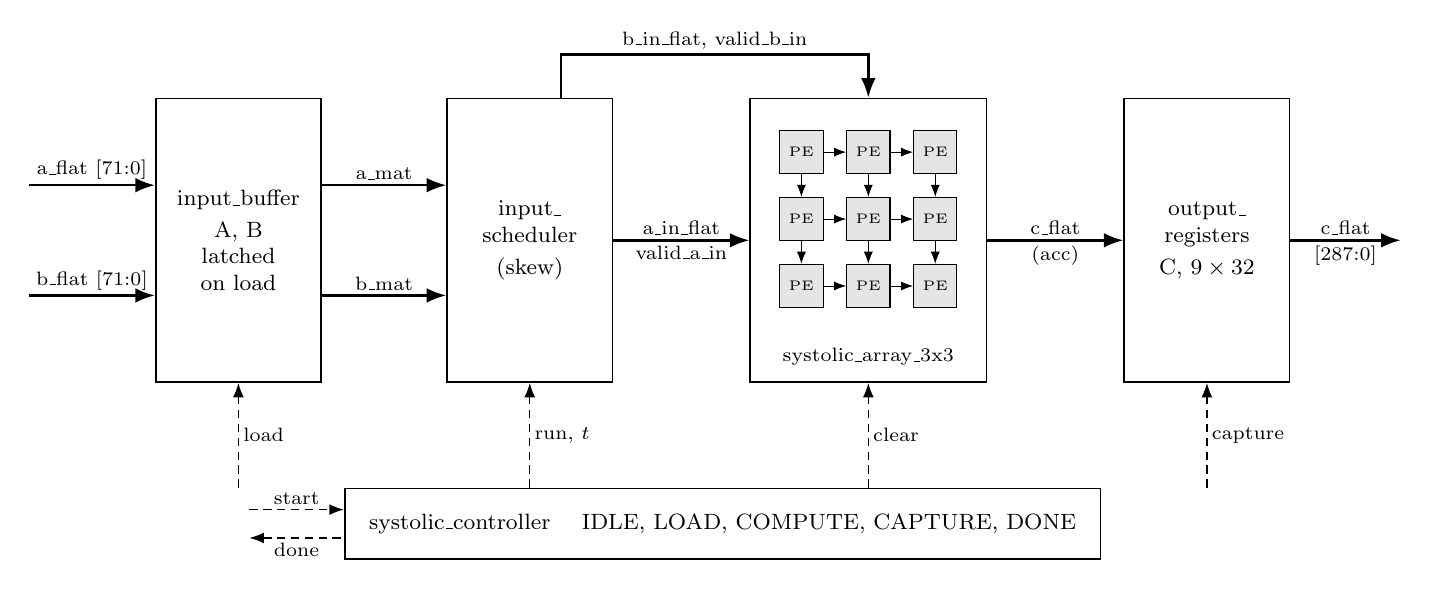
\begin{tikzpicture}[font=\footnotesize, >=Latex,
    blk/.style={draw, line width=0.6pt, minimum height=9mm, minimum width=21mm,
                align=center, fill=white},
    dat/.style={->, line width=0.9pt},
    ctl/.style={->, densely dashed, line width=0.5pt},
    lab/.style={font=\scriptsize, inner sep=1.5pt}]

  \node[blk, minimum height=36mm] (buf) at (0,0) {input\_buffer\\[2pt]A, B\\latched\\on load};
  \node[blk, minimum height=36mm] (sch) at (3.7,0) {input\_\\scheduler\\[2pt](skew)};
  \node[blk, minimum height=36mm, minimum width=30mm] (arr) at (8.0,0) {};
  \node[blk, minimum height=36mm] (out) at (12.3,0) {output\_\\registers\\[2pt]C, $9\times32$};
  \node[blk, minimum width=96mm] (ctrl) at (6.15,-3.6) {systolic\_controller \quad IDLE, LOAD, COMPUTE, CAPTURE, DONE};

  \foreach \i in {0,1,2} {
    \foreach \j in {0,1,2} {
      \node[draw, fill=black!10, minimum size=5.5mm, inner sep=0pt, font=\tiny]
        (pe\i\j) at ($(arr.center)+(-0.85+0.85*\j, 1.12-0.85*\i)$) {PE};
    }
  }
  \foreach \i in {0,1,2} {
    \draw[->, line width=0.3pt] (pe\i0) -- (pe\i1);
    \draw[->, line width=0.3pt] (pe\i1) -- (pe\i2);
    \draw[->, line width=0.3pt] (pe0\i) -- (pe1\i);
    \draw[->, line width=0.3pt] (pe1\i) -- (pe2\i);
  }
  \node[lab, anchor=north] at ($(arr.south)+(0,0.5)$) {systolic\_array\_3x3};

  % host side
  \draw[dat] ($(buf.west)+(-1.6,0.7)$) -- node[lab, above] {a\_flat [71:0]} ($(buf.west)+(0,0.7)$);
  \draw[dat] ($(buf.west)+(-1.6,-0.7)$) -- node[lab, above] {b\_flat [71:0]} ($(buf.west)+(0,-0.7)$);
  \draw[dat] (out.east) -- node[lab, above] {c\_flat} node[lab, below] {[287:0]} ++(1.4,0);

  % data path
  \draw[dat] ($(buf.east)+(0,0.7)$) -- node[lab, above] {a\_mat} ($(sch.west)+(0,0.7)$);
  \draw[dat] ($(buf.east)+(0,-0.7)$) -- node[lab, above] {b\_mat} ($(sch.west)+(0,-0.7)$);
  \draw[dat] (sch.east) -- node[lab, above] {a\_in\_flat} node[lab, below] {valid\_a\_in} (arr.west);
  \draw[dat] ($(sch.north)+(0.4,0)$) -- ++(0,0.55) -| node[lab, above, pos=0.25] {b\_in\_flat, valid\_b\_in} (arr.north);
  \draw[dat] (arr.east) -- node[lab, above] {c\_flat} node[lab, below] {(acc)} (out.west);

  % control
  \draw[ctl] (ctrl.north -| buf.south) -- node[lab, right] {load} (buf.south);
  \draw[ctl] (ctrl.north -| sch.south) -- node[lab, right] {run, $t$} (sch.south);
  \draw[ctl] (ctrl.north -| arr.south) -- node[lab, right] {clear} (arr.south);
  \draw[ctl] (ctrl.north -| out.south) -- node[lab, right] {capture} (out.south);
  \draw[ctl] ($(ctrl.west)+(-1.2,0.18)$) -- node[lab, above] {start} ($(ctrl.west)+(0,0.18)$);
  \draw[ctl, <-] ($(ctrl.west)+(-1.2,-0.18)$) -- node[lab, below] {done} ($(ctrl.west)+(0,-0.18)$);
\end{tikzpicture}
}
\caption{SysMAC top level. Solid arrows carry data; dashed arrows carry control signals from the controller.}
\label{fig:top}
\end{figure*}

\begin{figure*}[t]
\centering
\resizebox{0.9\textwidth}{!}{% Active cells of the 3 x 3 array at each step. PE(i,j) is active for
% i+j <= t <= i+j+2. The same pattern is checked against the RTL after
% every clock edge by tb_systolic_array.v.
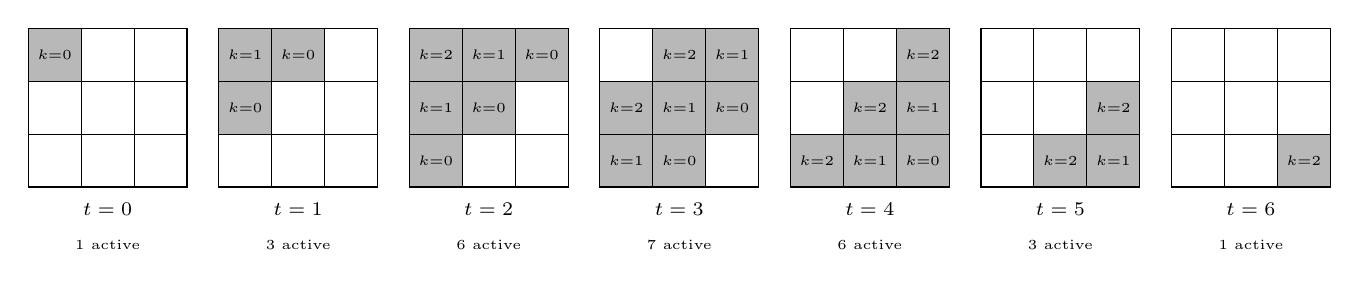
\begin{tikzpicture}[font=\scriptsize, x=0.42cm, y=0.42cm]
  \foreach \t in {0,...,6} {
    \begin{scope}[xshift=\t*2.42cm]
      \foreach \i in {0,1,2} {
        \foreach \j in {0,1,2} {
          \pgfmathtruncatemacro{\lo}{\i+\j}
          \pgfmathtruncatemacro{\hi}{\i+\j+2}
          \pgfmathtruncatemacro{\k}{\t-\i-\j}
          \ifnum\t<\lo
            \draw[line width=0.4pt] (\j*1.6,-\i*1.6) rectangle ++(1.6,-1.6);
          \else\ifnum\t>\hi
            \draw[line width=0.4pt] (\j*1.6,-\i*1.6) rectangle ++(1.6,-1.6);
          \else
            \draw[line width=0.4pt, fill=black!28] (\j*1.6,-\i*1.6) rectangle ++(1.6,-1.6);
            \node[font=\tiny] at (\j*1.6+0.8,-\i*1.6-0.8) {$k{=}\k$};
          \fi\fi
        }
      }
      \pgfmathtruncatemacro{\busy}{(\t<3) ? (\t+1)*(\t+2)/2 : ((\t==3) ? 7 : (7-\t)*(8-\t)/2)}
      \node[anchor=north] at (2.4,-5.0) {$t=\t$};
      \node[anchor=north, font=\tiny] at (2.4,-6.1) {\busy\ active};
    \end{scope}
  }
\end{tikzpicture}
}
\caption{Active cells in each compute cycle, with the index $k$ of the product each cell is computing.}
\label{fig:wave}
\end{figure*}

\subsubsection{Processing element}
Each cell (Fig.~\ref{fig:pe}) registers its two operands and their valid flags and forwards them to its right and lower neighbours. It adds the 16-bit product to its 32-bit accumulator only when both incoming valid flags are set. A \code{clear} signal, asserted while the matrices are loaded, resets every register in the cell, so no partial result can carry over between multiplications.

\begin{figure}[t]
\centering
\resizebox{0.8\columnwidth}{!}{% processing_element: four pass-through registers and one accumulator.
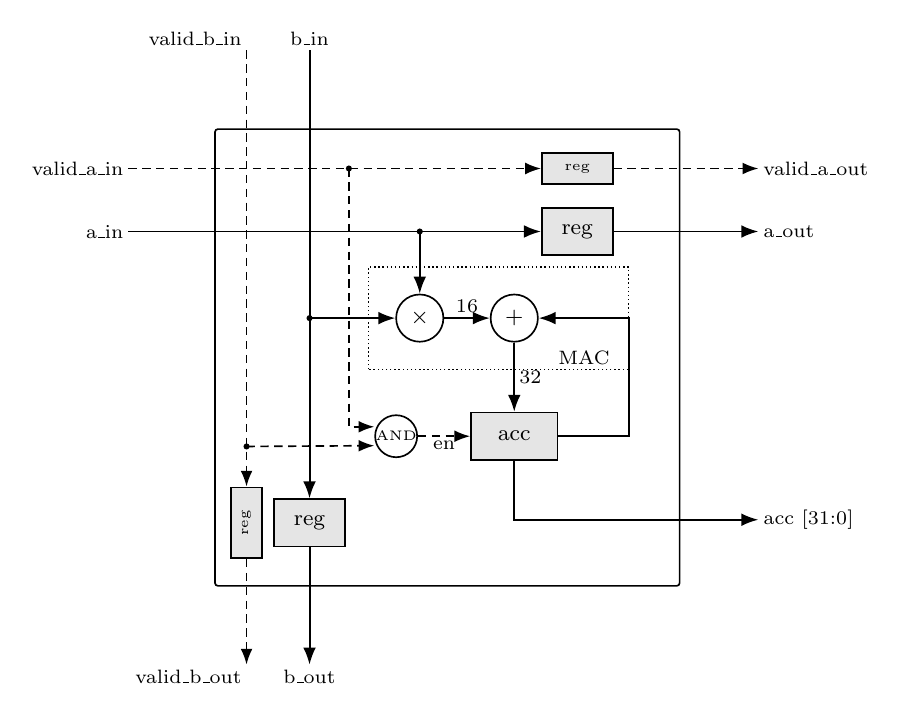
\begin{tikzpicture}[font=\footnotesize, >=Latex,
    reg/.style={draw, line width=0.6pt, minimum width=9mm, minimum height=6mm, fill=black!10},
    sreg/.style={draw, line width=0.6pt, minimum width=9mm, minimum height=4mm, fill=black!10, font=\tiny},
    op/.style={draw, circle, line width=0.6pt, minimum size=6mm, inner sep=0pt},
    w/.style={->, line width=0.7pt},
    v/.style={->, densely dashed, line width=0.6pt},
    lab/.style={font=\scriptsize, inner sep=1.5pt}]

  \draw[line width=0.6pt, rounded corners=1pt] (-2.3,-3.3) rectangle (3.6,2.5);

  % a and valid_a, left to right
  \node[sreg] (rva) at (2.3, 2.0) {reg};
  \node[reg]  (ra)  at (2.3, 1.2) {reg};
  \draw[v] (-3.4,2.0) node[lab, left] {valid\_a\_in} -- (rva.west);
  \draw[v] (rva.east) -- (4.6,2.0) node[lab, right] {valid\_a\_out};
  \draw[w] (-3.4,1.2) node[lab, left] {a\_in} -- (ra.west);
  \draw[w] (ra.east) -- (4.6,1.2) node[lab, right] {a\_out};

  % b and valid_b, top to bottom
  \node[reg]  (rb)  at (-1.1,-2.5) {reg};
  \node[sreg, rotate=90] (rvb) at (-1.9,-2.5) {reg};
  \draw[w] (-1.1,3.5) node[lab, above] {b\_in} -- (rb.north);
  \draw[w] (rb.south) -- (-1.1,-4.3) node[lab, below] {b\_out};
  \draw[v] (-1.9,3.5) node[lab, above left] {valid\_b\_in} -- (rvb.east);
  \draw[v] (rvb.west) -- (-1.9,-4.3) node[lab, below left] {valid\_b\_out};

  % MAC
  \node[op] (mul) at (0.3, 0.1) {$\times$};
  \node[op] (add) at (1.5, 0.1) {$+$};
  \node[reg, minimum width=11mm] (acc) at (1.5,-1.4) {acc};
  \node[op, minimum size=5mm, font=\tiny] (and) at (0.0,-1.4) {AND};
  \draw[w] (0.3,1.2) -- (mul.north);  \fill (0.3,1.2) circle (1.1pt);
  \draw[w] (-1.1,0.1) -- (mul.west);  \fill (-1.1,0.1) circle (1.1pt);
  \draw[w] (mul.east) -- node[lab, above] {16} (add.west);
  \draw[w] (add.south) -- node[lab, right] {32} (acc.north);
  \draw[w] (acc.east) -- ++(0.9,0) |- (add.east);
  \draw[w] (acc.south) -- ++(0,-0.75) -- ++(3.1,0) node[lab, right] {acc [31:0]};

  % accumulate enable
  \draw[v] (-0.6,2.0) |- ($(and.west)+(0,0.12)$);   \fill (-0.6,2.0) circle (1.1pt);
  \draw[v] (-1.9,-1.53) -- ($(and.west)+(0,-0.12)$); \fill (-1.9,-1.53) circle (1.1pt);
  \draw[v] (and.east) -- node[lab, below] {en} (acc.west);

  \draw[densely dotted, line width=0.5pt] (-0.35,-0.55) rectangle (2.95,0.75);
  \node[lab, anchor=south west] at (2.0,-0.55) {MAC};
\end{tikzpicture}
}
\caption{Processing element.}
\label{fig:pe}
\end{figure}

\subsubsection{Input skew}
Cell $(i,j)$ must receive $a_{ik}$ and $b_{kj}$ in the same cycle. A value entering row $i$ takes $j$ cycles to reach column $j$, and a value entering column $j$ takes $i$ cycles to reach row $i$. Delaying row $i$ of $A$ by $i$ cycles and column $j$ of $B$ by $j$ cycles aligns the pairs (Fig.~\ref{fig:array}). At compute cycle $t$ the scheduler therefore drives
\begin{equation}
\text{row } i:\; a_{i,\,t-i}, \qquad \text{column } j:\; b_{\,t-j,\,j},
\label{eq:skew}
\end{equation}
when the index lies in $\{0, 1, 2\}$, and zero with the valid flag cleared otherwise. The scheduler is purely combinational and is the only block that applies skew; the controller supplies only an enable and the cycle counter $t$.

\begin{figure}[t]
\centering
\resizebox{0.88\columnwidth}{!}{% 3 x 3 array with the skewed input streams drawn as a staircase.
% The element nearest the array enters first. Empty slots are zeros with
% valid low.
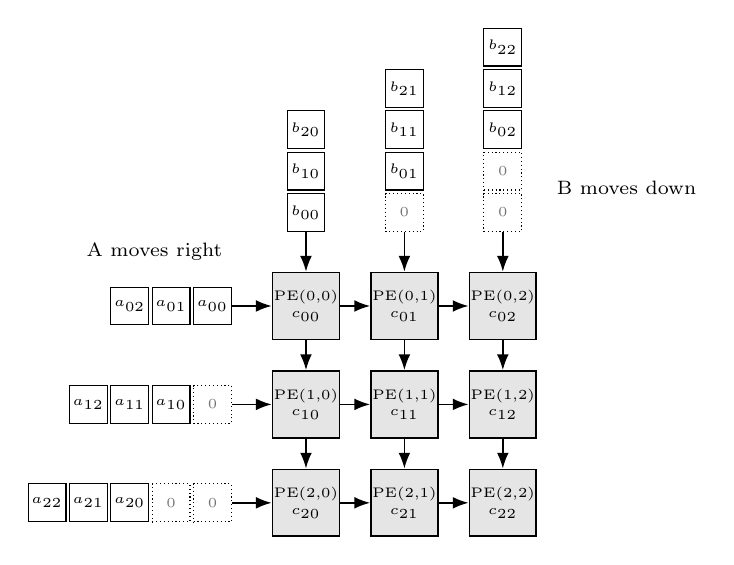
\begin{tikzpicture}[font=\scriptsize, >=Latex, x=1.25cm, y=1.25cm,
    pe/.style={draw, line width=0.6pt, minimum size=8.5mm, fill=black!10, align=center,
               inner sep=0pt, font=\tiny},
    tok/.style={draw, line width=0.4pt, minimum size=4.8mm, inner sep=0pt, font=\tiny},
    gap/.style={draw, densely dotted, line width=0.4pt, minimum size=4.8mm, inner sep=0pt,
                font=\tiny, text=black!55},
    w/.style={->, line width=0.6pt}]

  \foreach \i in {0,1,2} {
    \foreach \j in {0,1,2} {
      \node[pe] (p\i\j) at (\j,-\i) {PE(\i,\j)\\$c_{\i\j}$};
    }
  }
  \foreach \i in {0,1,2} {
    \draw[w] (p\i0) -- (p\i1);
    \draw[w] (p\i1) -- (p\i2);
    \draw[w] (p0\i) -- (p1\i);
    \draw[w] (p1\i) -- (p2\i);
  }

  % A streams on the left: row i has i empty slots before its first element
  \foreach \i in {0,1,2} {
    \foreach \s in {0,1,2,3,4} {
      \pgfmathtruncatemacro{\k}{\s-\i}
      \ifnum\k<0
        \node[gap] (a\i\s) at (-0.95-0.42*\s,-\i) {0};
      \else\ifnum\k<3
        \node[tok] (a\i\s) at (-0.95-0.42*\s,-\i) {$a_{\i\k}$};
      \fi\fi
    }
    \draw[w] (a\i0) -- (p\i0);
  }

  % B streams on the top: column j has j empty slots before its first element
  \foreach \j in {0,1,2} {
    \foreach \s in {0,1,2,3,4} {
      \pgfmathtruncatemacro{\k}{\s-\j}
      \ifnum\k<0
        \node[gap] (b\j\s) at (\j,0.95+0.42*\s) {0};
      \else\ifnum\k<3
        \node[tok] (b\j\s) at (\j,0.95+0.42*\s) {$b_{\k\j}$};
      \fi\fi
    }
    \draw[w] (b\j0) -- (p0\j);
  }

  \node[anchor=east, font=\scriptsize] at (-0.75,0.55) {A moves right};
  \node[anchor=west, font=\scriptsize] at (2.45,1.2) {B moves down};
\end{tikzpicture}
}
\caption{The array and its skewed input streams. The element nearest the array enters first; dotted slots are zeros with the valid flag cleared.}
\label{fig:array}
\end{figure}

\subsubsection{Controller}
The controller is a five-state Moore machine (Fig.~\ref{fig:fsm}). LOAD latches the inputs and clears the array in one cycle, and COMPUTE lasts seven cycles. CAPTURE is needed because the final product is added on the clock edge that ends COMPUTE, so the accumulators are complete only one cycle later. DONE asserts \code{done} for one cycle while the result is on the output. A \code{start} pulse outside IDLE is ignored. Fig.~\ref{fig:timing} shows one complete multiplication.

\begin{figure}[t]
\centering
\resizebox{0.85\columnwidth}{!}{% systolic_controller state machine. Outputs are Moore: each depends only on the state.
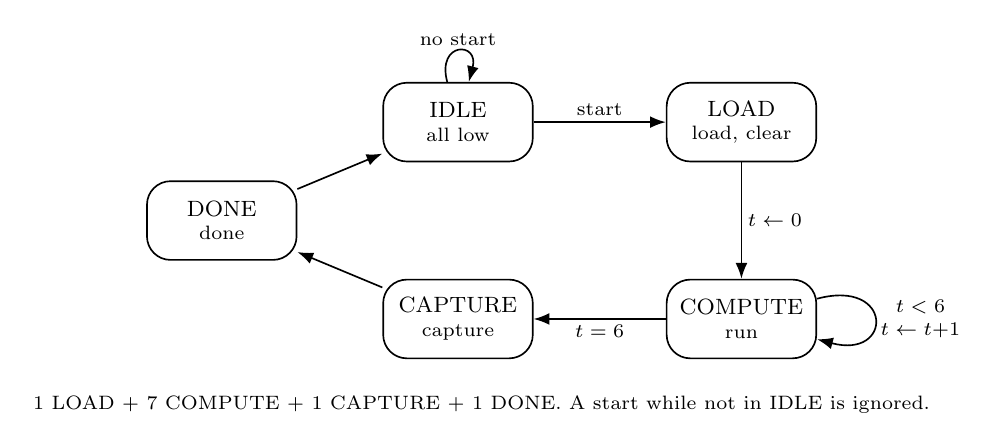
\begin{tikzpicture}[font=\footnotesize, >=Latex,
    st/.style={draw, line width=0.6pt, rounded corners=3mm, minimum width=19mm,
               minimum height=10mm, align=center, fill=white},
    tr/.style={->, line width=0.6pt},
    lab/.style={font=\scriptsize, inner sep=2pt, align=center}]

  \node[st] (idle) at (0,0)      {IDLE\\[-1pt]{\scriptsize all low}};
  \node[st] (load) at (3.6,0)    {LOAD\\[-1pt]{\scriptsize load, clear}};
  \node[st] (comp) at (3.6,-2.5) {COMPUTE\\[-1pt]{\scriptsize run}};
  \node[st] (cap)  at (0,-2.5)   {CAPTURE\\[-1pt]{\scriptsize capture}};
  \node[st] (done) at (-3.0,-1.25) {DONE\\[-1pt]{\scriptsize done}};

  \draw[tr] (idle) -- node[lab, above] {start} (load);
  \draw[tr] (load) -- node[lab, right] {$t \leftarrow 0$} (comp);
  \draw[tr] (comp) -- node[lab, below] {$t = 6$} (cap);
  \draw[tr] (cap)  -- (done);
  \draw[tr] (done) -- (idle);
  \draw[tr] (comp) edge[loop right, looseness=5] node[lab, right] {$t < 6$\\$t \leftarrow t{+}1$} (comp);
  \draw[tr] (idle) edge[loop above, looseness=5] node[lab, above] {no start} (idle);

  \node[lab, anchor=north] at (0.3,-3.4)
    {1 LOAD + 7 COMPUTE + 1 CAPTURE + 1 DONE. A start while not in IDLE is ignored.};
\end{tikzpicture}
}
\caption{Controller state machine and its outputs.}
\label{fig:fsm}
\end{figure}

\begin{figure}[t]
\centering
\resizebox{\columnwidth}{!}{% One job, cycle by cycle. Edge 1 samples start; done is visible after edge 10.
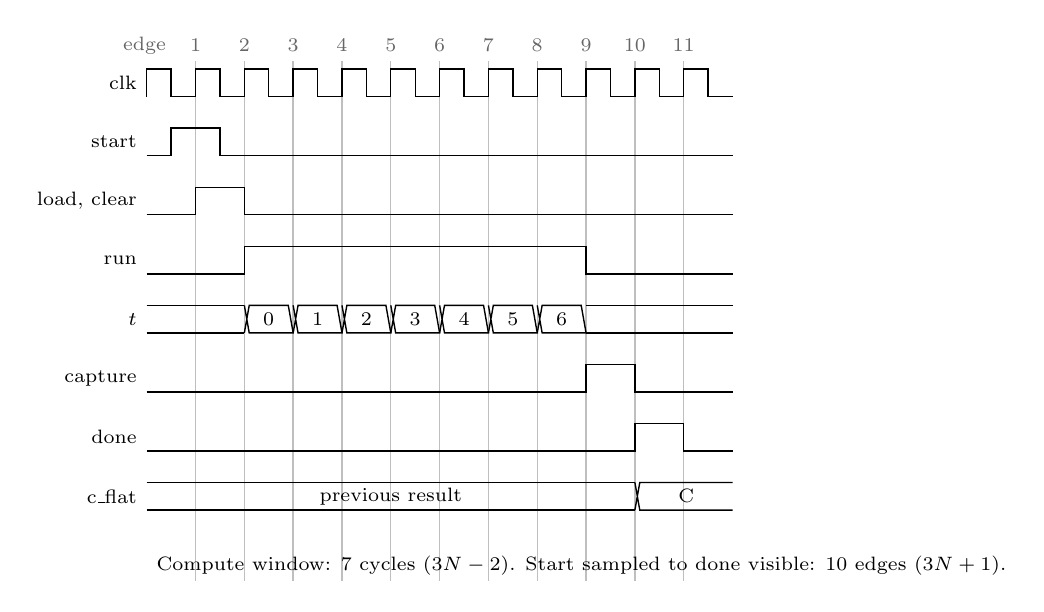
\begin{tikzpicture}[font=\scriptsize, x=0.62cm, y=0.5cm, line width=0.5pt]
  \def\lo{0} \def\hi{0.7}
  % cycle grid: cycle c spans [c, c+1], edge e sits at x = e
  \foreach \e in {1,...,11} {
    \draw[black!25] (\e,0.9) -- (\e,-12.3);
    \node[black!60] at (\e,1.3) {\e};
  }
  \node[anchor=east, black!60] at (0.6,1.3) {edge};

  % helper: a signal high from x1 to x2 on row y
  \newcommand{\sig}[4]{% name, y, x1, x2
    \node[anchor=east] at (0,#2+0.35) {#1};
    \draw (0,#2) -- (#3,#2) -- (#3,#2+\hi) -- (#4,#2+\hi) -- (#4,#2) -- (12,#2);}

  % clock
  \node[anchor=east] at (0,0.35) {clk};
  \foreach \c in {0,...,11} {
    \draw (\c,0) -- (\c,\hi) -- (\c+0.5,\hi) -- (\c+0.5,0) -- (\c+1,0);
  }
  \sig{start}{-1.5}{0.5}{1.5}
  \sig{load, clear}{-3}{1}{2}
  \sig{run}{-4.5}{2}{9}
  % t bus
  \node[anchor=east] at (0,-5.65) {$t$};
  \draw (0,-6) -- (2,-6) (0,-5.3) -- (2,-5.3);
  \foreach \c in {2,...,8} {
    \pgfmathtruncatemacro{\tv}{\c-2}
    \draw (\c,-6) -- (\c+0.1,-5.3) -- (\c+0.9,-5.3) -- (\c+1,-6) -- (\c+0.1,-6) -- (\c,-5.3);
    \node at (\c+0.5,-5.65) {\tv};
  }
  \draw (9,-6) -- (12,-6) (9,-5.3) -- (12,-5.3);
  \sig{capture}{-7.5}{9}{10}
  \sig{done}{-9}{10}{11}
  % c_flat bus
  \node[anchor=east] at (0,-10.15) {c\_flat};
  \draw (0,-10.5) -- (10,-10.5) (0,-9.8) -- (10,-9.8);
  \draw (10,-10.5) -- (10.1,-9.8) -- (12,-9.8) (10,-9.8) -- (10.1,-10.5) -- (12,-10.5);
  \node at (5,-10.15) {previous result};
  \node at (11.05,-10.15) {C};

  \node[anchor=west, align=left] at (0,-11.9)
    {Compute window: 7 cycles ($3N-2$). Start sampled to done visible: 10 edges ($3N+1$).};
\end{tikzpicture}
}
\caption{One multiplication. Edge 1 samples \code{start}; \code{done} and the result are visible after edge 10.}
\label{fig:timing}
\end{figure}


\subsection{Timing analysis}
\label{sec:timing}
From \eqref{eq:skew}, cell $(i,j)$ computes its $k$-th product at
\begin{equation}
t = i + j + k .
\label{eq:when}
\end{equation}
The last product, at cell $(2,2)$ with $k = 2$, occurs at $t = 3(N-1) = 6$, so the computation takes $3N - 2 = 7$ cycles. The active cells form a diagonal wavefront (Fig.~\ref{fig:wave}). Counting from the edge that samples \code{start} to the edge after which \code{done} is visible, a multiplication takes
\begin{equation}
1 + 1 + (3N-2) + 1 = 3N + 1 = 10 \text{ cycles}.
\end{equation}

SCALE-Sim models the output-stationary runtime as $2S_R + S_C + T - 2$ for $S_R$ rows, $S_C$ columns and $T$ accumulation steps~\cite{scalesim2020}. For a $3 \times 3$ multiplication this gives $4N - 2 = 10$: our seven compute cycles plus $N = 3$ cycles to shift results out through the bottom edge. SysMAC reads all accumulators in parallel instead, so the two models agree once the readout method is taken into account.

\emph{Utilisation.} Only $N^3 = 27$ of the $N^2(3N-2) = 63$ cell-cycles perform useful work, a utilisation of 42.9\%. Cells are idle while the wavefront fills and drains the array. The fraction approaches one third as $N$ grows; overlapping successive multiplications is the standard remedy.

\subsection{Accumulator width}
With signed 8-bit operands, the product of largest magnitude is $(-128)^2 = 16\,384$, which is positive. The largest sum of three products is therefore $49\,152$, while the most negative, $3 \times (-128 \times 127) = -48\,768$, is smaller in magnitude. Representing $49\,152$ requires 17 signed bits. In general, $W$-bit operands require
\begin{equation}
B_{\min} = 2W + \lfloor \log_2 N \rfloor
\end{equation}
bits, one fewer than the commonly quoted $2W + \lceil \log_2 N \rceil$ when $N$ is not a power of two. SysMAC uses 32 bits, following the TPU and integer inference practice~\cite{jouppi2017, jacob2018}; the extra width allows accumulation over larger, tiled matrices.

\subsection{Sequential baseline}
The baseline evaluates \eqref{eq:matmul} with one MAC unit and three counters, performing one MAC per cycle. It has the same ports and handshake as the systolic design: one LOAD cycle, 27 compute cycles and one DONE cycle, for a latency of 29 cycles in the same convention. The systolic array is thus $2.9\times$ faster in cycles while using nine multipliers instead of one. Because a comparison in cycles alone favours the array, Section~\ref{sec:future} adds clock frequency and area as future work.

\subsection{Verification method}
\label{sec:verif}
\emph{Reference model.} An independent Python model contains three descriptions of the computation: the triple loop of \eqref{eq:matmul}; a register-level model of the array, advanced one clock edge at a time and tracking both valid flags; and the operation order of the baseline. Before producing any test data, it checks that the three agree with each other and with NumPy on 1560 matrix pairs for $N \in \{2, 3, 4, 5, 8\}$, and that every cell is active exactly in the cycles given by \eqref{eq:when}.

\emph{Test data.} The model produces 112 test cases: 12 directed and 100 random. The directed cases cover zero matrices, the identity on either side, all elements equal to $-128$ or $127$, $-128$ against $127$, alternating signs, a single non-zero element in either corner, and an asymmetric pair that fails if $B$ is read transposed. For each case the model also records the expected scheduler output in every cycle and the value of every accumulator after every clock edge.

\emph{Testbenches.} Verification proceeds bottom-up, with one testbench per level:
\begin{enumerate}
\item \emph{Units:} the MAC unit and processing element, with directed cases for signs, valid flags, clear and reset.
\item \emph{Scheduler and array:} scheduler outputs against the expected table for $t = 0, \ldots, 6$; array accumulators against the model after every clock edge, for $N = 2, 3, 4$.
\item \emph{Controller:} the state sequence, the seven values of $t$ and the one-cycle \code{done} pulse.
\item \emph{System:} directed, random and back-to-back multiplications without intermediate reset, an exact latency check, and a reset during computation. A second system testbench changes the inputs immediately after LOAD, so a design that fails to latch them is detected, and issues a second \code{start} during computation, which must be ignored.
\end{enumerate}
A single script regenerates the test data and runs every testbench with Icarus Verilog.

% ======================================================================
\section{Results}
\label{sec:results}

\subsection{Functional correctness}
All nine testbenches pass on the integrated design (Table~\ref{tab:tests}). The system testbenches measure exactly 10 cycles from start to done for every multiplication, and the baseline measures 29 cycles on the same 112 cases. The demonstration case, $A = [[1,2,3],[4,5,6],[7,8,9]]$ and $B = [[9,8,7],[6,5,4],[3,2,1]]$, produces $C = [[30,24,18],[84,69,54],[138,114,90]]$.

\begin{table}[t]
\caption{Testbench results on the integrated design}
\label{tab:tests}
\centering
\begin{tabular}{@{}lp{0.5\columnwidth}@{}}
\toprule
Testbench & Result \\
\midrule
MAC unit & pass \\
Processing element & pass \\
Input scheduler & pass \\
Array & pass for $N = 2, 3, 4$; 112 cases cycle by cycle \\
Controller & pass \\
System & pass, 109 cases, 10 cycles \\
Demonstration & pass \\
Vector test, systolic & pass, 112 cases, 10 cycles \\
Vector test, baseline & pass, 112 cases, 29 cycles \\
\bottomrule
\end{tabular}
\end{table}

\subsection{Strength of the tests}
A passing test is evidence of correctness only if it would fail on an incorrect design. We therefore introduced one error at a time into a copy of the integrated design and reran all testbenches (Table~\ref{tab:mut}). Every error was detected, most by four independent testbenches. The unlatched input buffer was detected only by the vector testbench, the only one that changes the inputs after LOAD. One change was not detected: output registers that copy the accumulators on every cycle rather than only on \code{capture}. This does not violate the specification, because the accumulators are stable after the computation ends and the output is only guaranteed while \code{done} is asserted.

\begin{table}[t]
\caption{Planted design errors and the testbenches that detect them}
\label{tab:mut}
\centering
\begin{tabular}{@{}lp{0.47\columnwidth}@{}}
\toprule
Planted error & Detected by \\
\midrule
$B$ enters one cycle late & scheduler, system, demo, vector \\
$B$ read transposed & scheduler, system, demo, vector \\
unsigned multiplication & PE, array, system, vector \\
16-bit accumulator & PE, array, system, vector \\
no clear between runs & PE, array, system, vector \\
controller ends one cycle early & controller, system, demo, vector \\
inputs not latched & vector \\
\bottomrule
\end{tabular}
\end{table}

\subsection{Performance and resources}
Table~\ref{tab:perf} compares the two designs. The array completes a multiplication in 10 cycles against 29. A preliminary synthesis with Yosys 0.71 for Xilinx 7-series primitives reports no latches or structural problems. The baseline requires more lookup tables than the array, because it must select one of nine operands every cycle. These figures are cell counts without timing.

\begin{table}[t]
\caption{Systolic array and sequential baseline}
\label{tab:perf}
\centering
\begin{tabular}{@{}lrr@{}}
\toprule
 & Systolic & Baseline \\
\midrule
Multipliers & 9 & 1 \\
Compute cycles & 7 & 27 \\
Start to done (cycles) & 10 & 29 \\
DSP48E1 blocks & 9 & 1 \\
Flip-flops & 602 & 474 \\
LUTs & 144 & 408 \\
\bottomrule
\end{tabular}
\end{table}

% ======================================================================
\section{Limitations and Future Work}
\label{sec:future}
The cycle comparison favours the array, which uses nine multipliers to obtain a $2.9\times$ reduction in cycles; a fair comparison also requires clock frequency and area. We will therefore synthesise and implement both designs with Vivado to obtain utilisation, maximum frequency and the area-time product. Utilisation is limited to 42.9\% by the fill and drain of the wavefront; overlapping successive multiplications would raise it. If the combined multiply-add path limits the clock frequency, a registered multiplier in each cell would shorten it at the cost of one cycle of latency.

% ======================================================================
\section{Individual Contributions}
\label{sec:contrib}
\begin{center}
\begin{tabular}{@{}lp{0.68\columnwidth}@{}}
\toprule
Member & Contribution \\
\midrule
Abhishek Rana & MAC unit and processing element, with their testbenches \\
Harshil Valecha & Port specification, controller, top-level integration, controller, system and demonstration testbenches, repository and code review \\
Sushant Yadav & Parameterised $N \times N$ array with $3 \times 3$ wrapper, and its testbench for $N = 2, 3, 4$ \\
Piyush & Input buffer, input scheduler, output registers, scheduler testbench \\
Priyanshu Tomar & Reference model and test data, simulation script, sequential baseline and vector testbench, mutation testing, block diagrams, README, report \\
\bottomrule
\end{tabular}
\end{center}

\begin{thebibliography}{00}
\bibitem{kung1978} H. T. Kung and C. E. Leiserson, ``Systolic arrays (for VLSI),'' in \emph{Sparse Matrix Proceedings 1978}, I. S. Duff and G. W. Stewart, Eds. Philadelphia, PA, USA: SIAM, 1979, pp. 256-282.
\bibitem{kung1982} H. T. Kung, ``Why systolic architectures?,'' \emph{Computer}, vol. 15, no. 1, pp. 37-46, Jan. 1982, doi: 10.1109/MC.1982.1653825.
\bibitem{jouppi2017} N. P. Jouppi \emph{et al.}, ``In-datacenter performance analysis of a tensor processing unit,'' in \emph{Proc. 44th Annu. Int. Symp. Comput. Archit. (ISCA)}, 2017, pp. 1-12, doi: 10.1145/3079856.3080246.
\bibitem{jacob2018} B. Jacob \emph{et al.}, ``Quantization and training of neural networks for efficient integer-arithmetic-only inference,'' in \emph{Proc. IEEE/CVF Conf. Comput. Vis. Pattern Recognit. (CVPR)}, 2018, pp. 2704-2713, doi: 10.1109/CVPR.2018.00286.
\bibitem{eyeriss2016} Y.-H. Chen, J. Emer, and V. Sze, ``Eyeriss: A spatial architecture for energy-efficient dataflow for convolutional neural networks,'' in \emph{Proc. 43rd Annu. Int. Symp. Comput. Archit. (ISCA)}, 2016, pp. 367-379, doi: 10.1109/ISCA.2016.40.
\bibitem{sze2017} V. Sze, Y.-H. Chen, T.-J. Yang, and J. S. Emer, ``Efficient processing of deep neural networks: A tutorial and survey,'' \emph{Proc. IEEE}, vol. 105, no. 12, pp. 2295-2329, Dec. 2017, doi: 10.1109/JPROC.2017.2761740.
\bibitem{scalesim2018} A. Samajdar, Y. Zhu, P. Whatmough, M. Mattina, and T. Krishna, ``SCALE-Sim: Systolic CNN accelerator simulator,'' arXiv:1811.02883, 2018.
\bibitem{scalesim2020} A. Samajdar, J. M. Joseph, Y. Zhu, P. Whatmough, M. Mattina, and T. Krishna, ``A systematic methodology for characterizing scalability of DNN accelerators using SCALE-Sim,'' in \emph{Proc. IEEE Int. Symp. Perform. Anal. Syst. Softw. (ISPASS)}, 2020, pp. 58-68.
\bibitem{gemmini2021} H. Genc \emph{et al.}, ``Gemmini: Enabling systematic deep-learning architecture evaluation via full-stack integration,'' in \emph{Proc. 58th ACM/IEEE Design Autom. Conf. (DAC)}, 2021, pp. 769-774, doi: 10.1109/DAC18074.2021.9586216.
\end{thebibliography}

\end{document}
